\chapter{Технологический раздел}

В данном разделе выбраны средства реализации, приведена структура программы и описание классов, продемонстрирован интерфейс программы.

\section{Выбор средств реализации}

В качестве языка программирования был выбран С++ \cite{cpp-lang}, так как:
\begin{itemize}[label=---]
\item Я ознакомился с этим языком в рамках курса по ООП.
\item Данный язык программирования поддерживает \linebreak объектно-ориентированную модель разработки, что позволяет четко структурировать программу.
\item Язык C++ поддерживает многопоточность и предоставляет встроенные средства для осуществления замеров времени работы.
\end{itemize}

В качестве графического фреймворка был выбран Qt \cite{qt}, так как этот фреймворк поддерживает Qt Designer, приложение для разработки UI и предоставляет множество средств для отображения визуальной сцены на виджете в приложении.

В качестве среды разработки была выбрана <<Microsoft Visual Studio>> \cite{vs}, так как:

\begin{itemize}[label=---]
\item Для студентов это ПО распространяется бесплатно.
\item Эта среда разработки поддерживает интеграцию с Qt.
\item Она имеет встроенную технологию автодополнения IntelliSense\cite{intelli}, позволяющую сильно облегчить процесс разработки.
\item Имеет встроенный отладчик.
\end{itemize}

\section{Структура программы}

Схема UML классов моей программы изображена на рисунке \ref{fig:uml}. Приведенная схема отображает отношения между кассами и их интерфейс.

\begin{figure}[h]
	\centering
	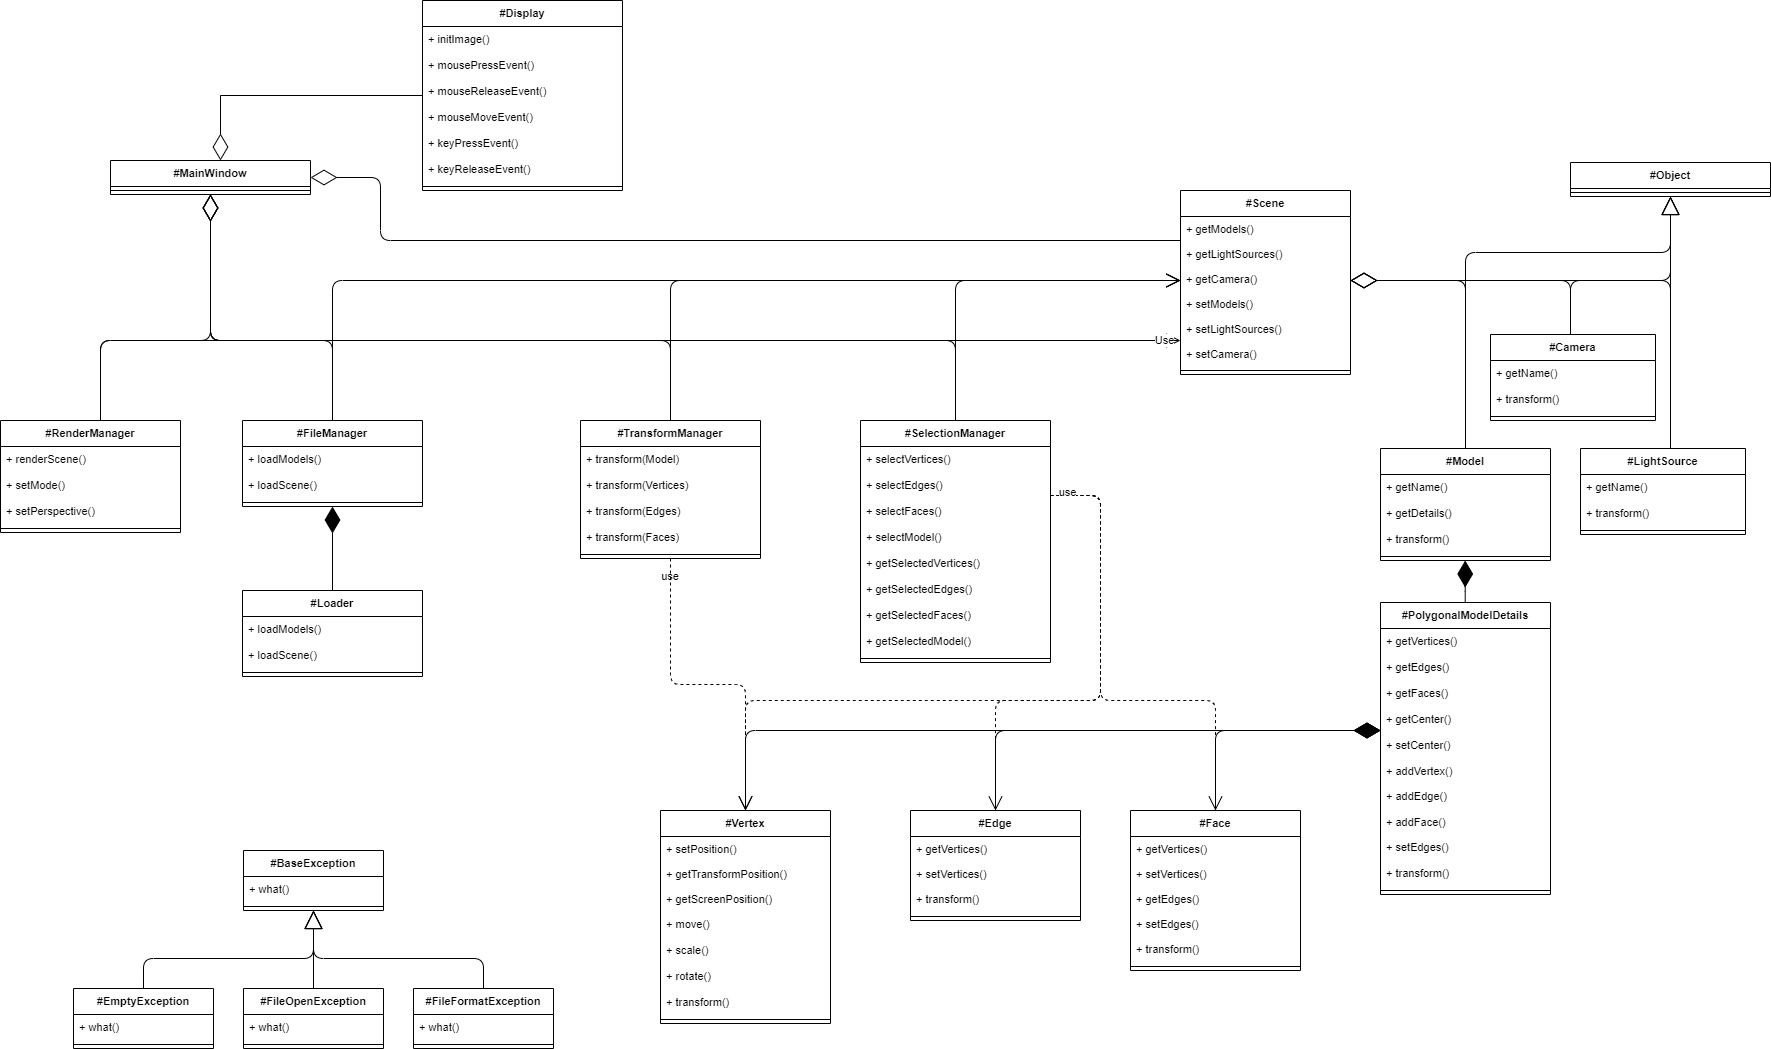
\includegraphics[scale=0.4, angle=-90]{inc/img/uml.jpg}
	\caption{UML-схема классов}
	\label{fig:uml}
\end{figure} 

\clearpage

\section{Описание классов и модулей программы}

\textbf{Интерфейс:}
\begin{itemize}[label=---]
\item MainWindow (MainWindow.h, MainWindow.cpp) – класс, описывающий интерфейс главного окна приложения. Наследуется от QMainWindow;
\item Display (Display.h, Display.cpp) – класс, описывающий виджет для отображения буфера кадра. Наследуется от QWidget;
\item MainWindow.ui – форма пользовательского интерфейса главного окна приложения.
\end{itemize}


\textbf{Сцена:} 

Scene (Scene.h, Scene.cpp) – класс, описывающий сцену. Этот класс является контейнером для хранения объектов сцены: источников света, моделей и камеры.

\textbf{Объекты сцены:}
\begin{itemize}[label=---]
\item Object (Object.h) – абстрактный класс объекта;
\item LightSource (LightSource.h, LightSource.cpp) – класс, описывающий точечный источник освещения;
\item Camera (Camera.h, Camera.cpp) – класс, описывающий камеру;
\item Model (Model.h, Model.cpp) – класс, описывающий трехмерную модель.
\end{itemize}

\textbf{Составляющие части модели:}
\begin{itemize}[label=---]
\item Vertex (Vertex.h, Vertex.cpp) – класс, описывающий вершину модели;
\item Edge (Edge.h, Edge.cpp) – класс, описывающий ребро модели;
\item Face (Face.h, Face.cpp) – класс, описывающий грань модели;
\item PolygonalModelDetails (PolygonalModelDetails.h, PolygonalModelDetails.cpp) – класс, описывающий реализацию полигональной модели.
\end{itemize}

\textbf{Менеджеры:}
\begin{itemize}[label=---]
\item TransformManager (TransformManager.h, TransformManager.cpp) – класс, описывающий менеджера трансформации. Этот менеджер осуществляет за перенос, поворот и масштабирование моделей и их составляющих частей;
\item FileManager (FileManager.h, FileManager.cpp) – класс, описывающий менеджера работы с файлами. Этот менеджер осуществляет загрузку сцены из файла и ее сохранение;
\item RenderManager (RenderManager.h, RenderManager.cpp) – класс, описывающий менеджера отрисовки. Этот менеджер осуществляет отрисовку сцены в буфер кадра;
\item SelectionManager (SelectionManager.h, SelectionManager.cpp) – класс, описывающий менеджера выбора. Этот менеджер отвечает за выбор моделей и их составляющих частей на дисплее.
\end{itemize}

\textbf{Работа с файлами:} 

Loader (Loader.h, Loader.cpp) – класс, осуществляющий загрузку из файла и валидацию сцены.

\section{Реализации алгоритмов}

В листингах \ref{lst:process_rect}, \ref{lst:process_face} представлена реализация алгоритмов обработки пикселей обрамляющего прямоугольника и многопоточной обработки грани модели.\clearpage

\begin{center}
	\captionsetup{justification=raggedright,singlelinecheck=off}
	\begin{lstlisting}[label=lst:process_rect,caption=Реализация алгоритма обработки пикселей обрамляющего прямоугольника]
		void RenderManager::processFramingRectPixel(
		unique_ptr<ThreadParams> params
		) {
			int startY = params->startY;
			int stopY = params->stopY;
			int startX = params->startX;
			int stopX = params->stopX;
			
			const ScreenFace& face = params->face;
			double square = params->square;
			const QRgb& color = params->color;
			const shared_ptr<Face>& basicFace = params->basicFace;
			const shared_ptr<Model>& model = params->model;
			
			for (int y = startY; y <= stopY; y++) {
				for (int x = startX; x <= stopX; x++) {
					
					auto barCoords = calculateBarycentric(QPoint(x, y), face, square);
					
					if (barCoords.x() >= -EPS && barCoords.y() >= -EPS && barCoords.z() >= -EPS) {
						double z = baryCentricInterpolation(face[0], face[1], face[2], barCoords);
						
						this->processPixel(x, y, z, color);
						this->updateFaceBuffer(Vector2d(x, y), z, basicFace);
						this->updateModelBuffer(Vector2d(x, y), z, model);
					}
				}
			}
		}
	\end{lstlisting}
\end{center}

\clearpage

\begin{center}
	\captionsetup{justification=raggedright,singlelinecheck=off}
	\begin{lstlisting}[label=lst:process_face,caption=Реализация алгоритма обработки грани в несколько потоков]
		void RenderManager::processFace(
		const ScreenFace& face, const QRect& framingRect, 
		const QRgb& color, const shared_ptr<Face>& basicFace, 
		const shared_ptr<Model>& model
		) {
			double square = (face[0].y() - face[2].y()) * (face[1].x() - face[2].x()) +
			(face[1].y() - face[2].y()) * (face[2].x() - face[0].x());
			
			int threadCount = config.threadCount;
			vector<thread> threads(threadCount);
			
			double startY = framingRect.top();
			double stepY = (framingRect.bottom() - framingRect.top()) / double(threadCount);
			
			for (auto& thread : threads) {
				unique_ptr<ThreadParams> params = unique_ptr<ThreadParams>(new ThreadParams{
					0, 0, framingRect.left(), framingRect.right(), face, square, color, basicFace, model
				});
				
				params->startY = round(startY);
				params->stopY = round(startY + stepY);
				thread = std::thread(
				&RenderManager::processFramingRectPixel, 
				this, move(params));
				
				startY += stepY;
			}
			
			for (auto& thread : threads) {
				thread.join();
			}
			
		\end{lstlisting}
	\end{center}

\section{Интерфейс программы}

Главное окно программы (рисунок \ref{fig:interface}) имеет несколько виджетов на которых располагаются основные элементы интерфейса:

\begin{figure}[h]
	\centering
	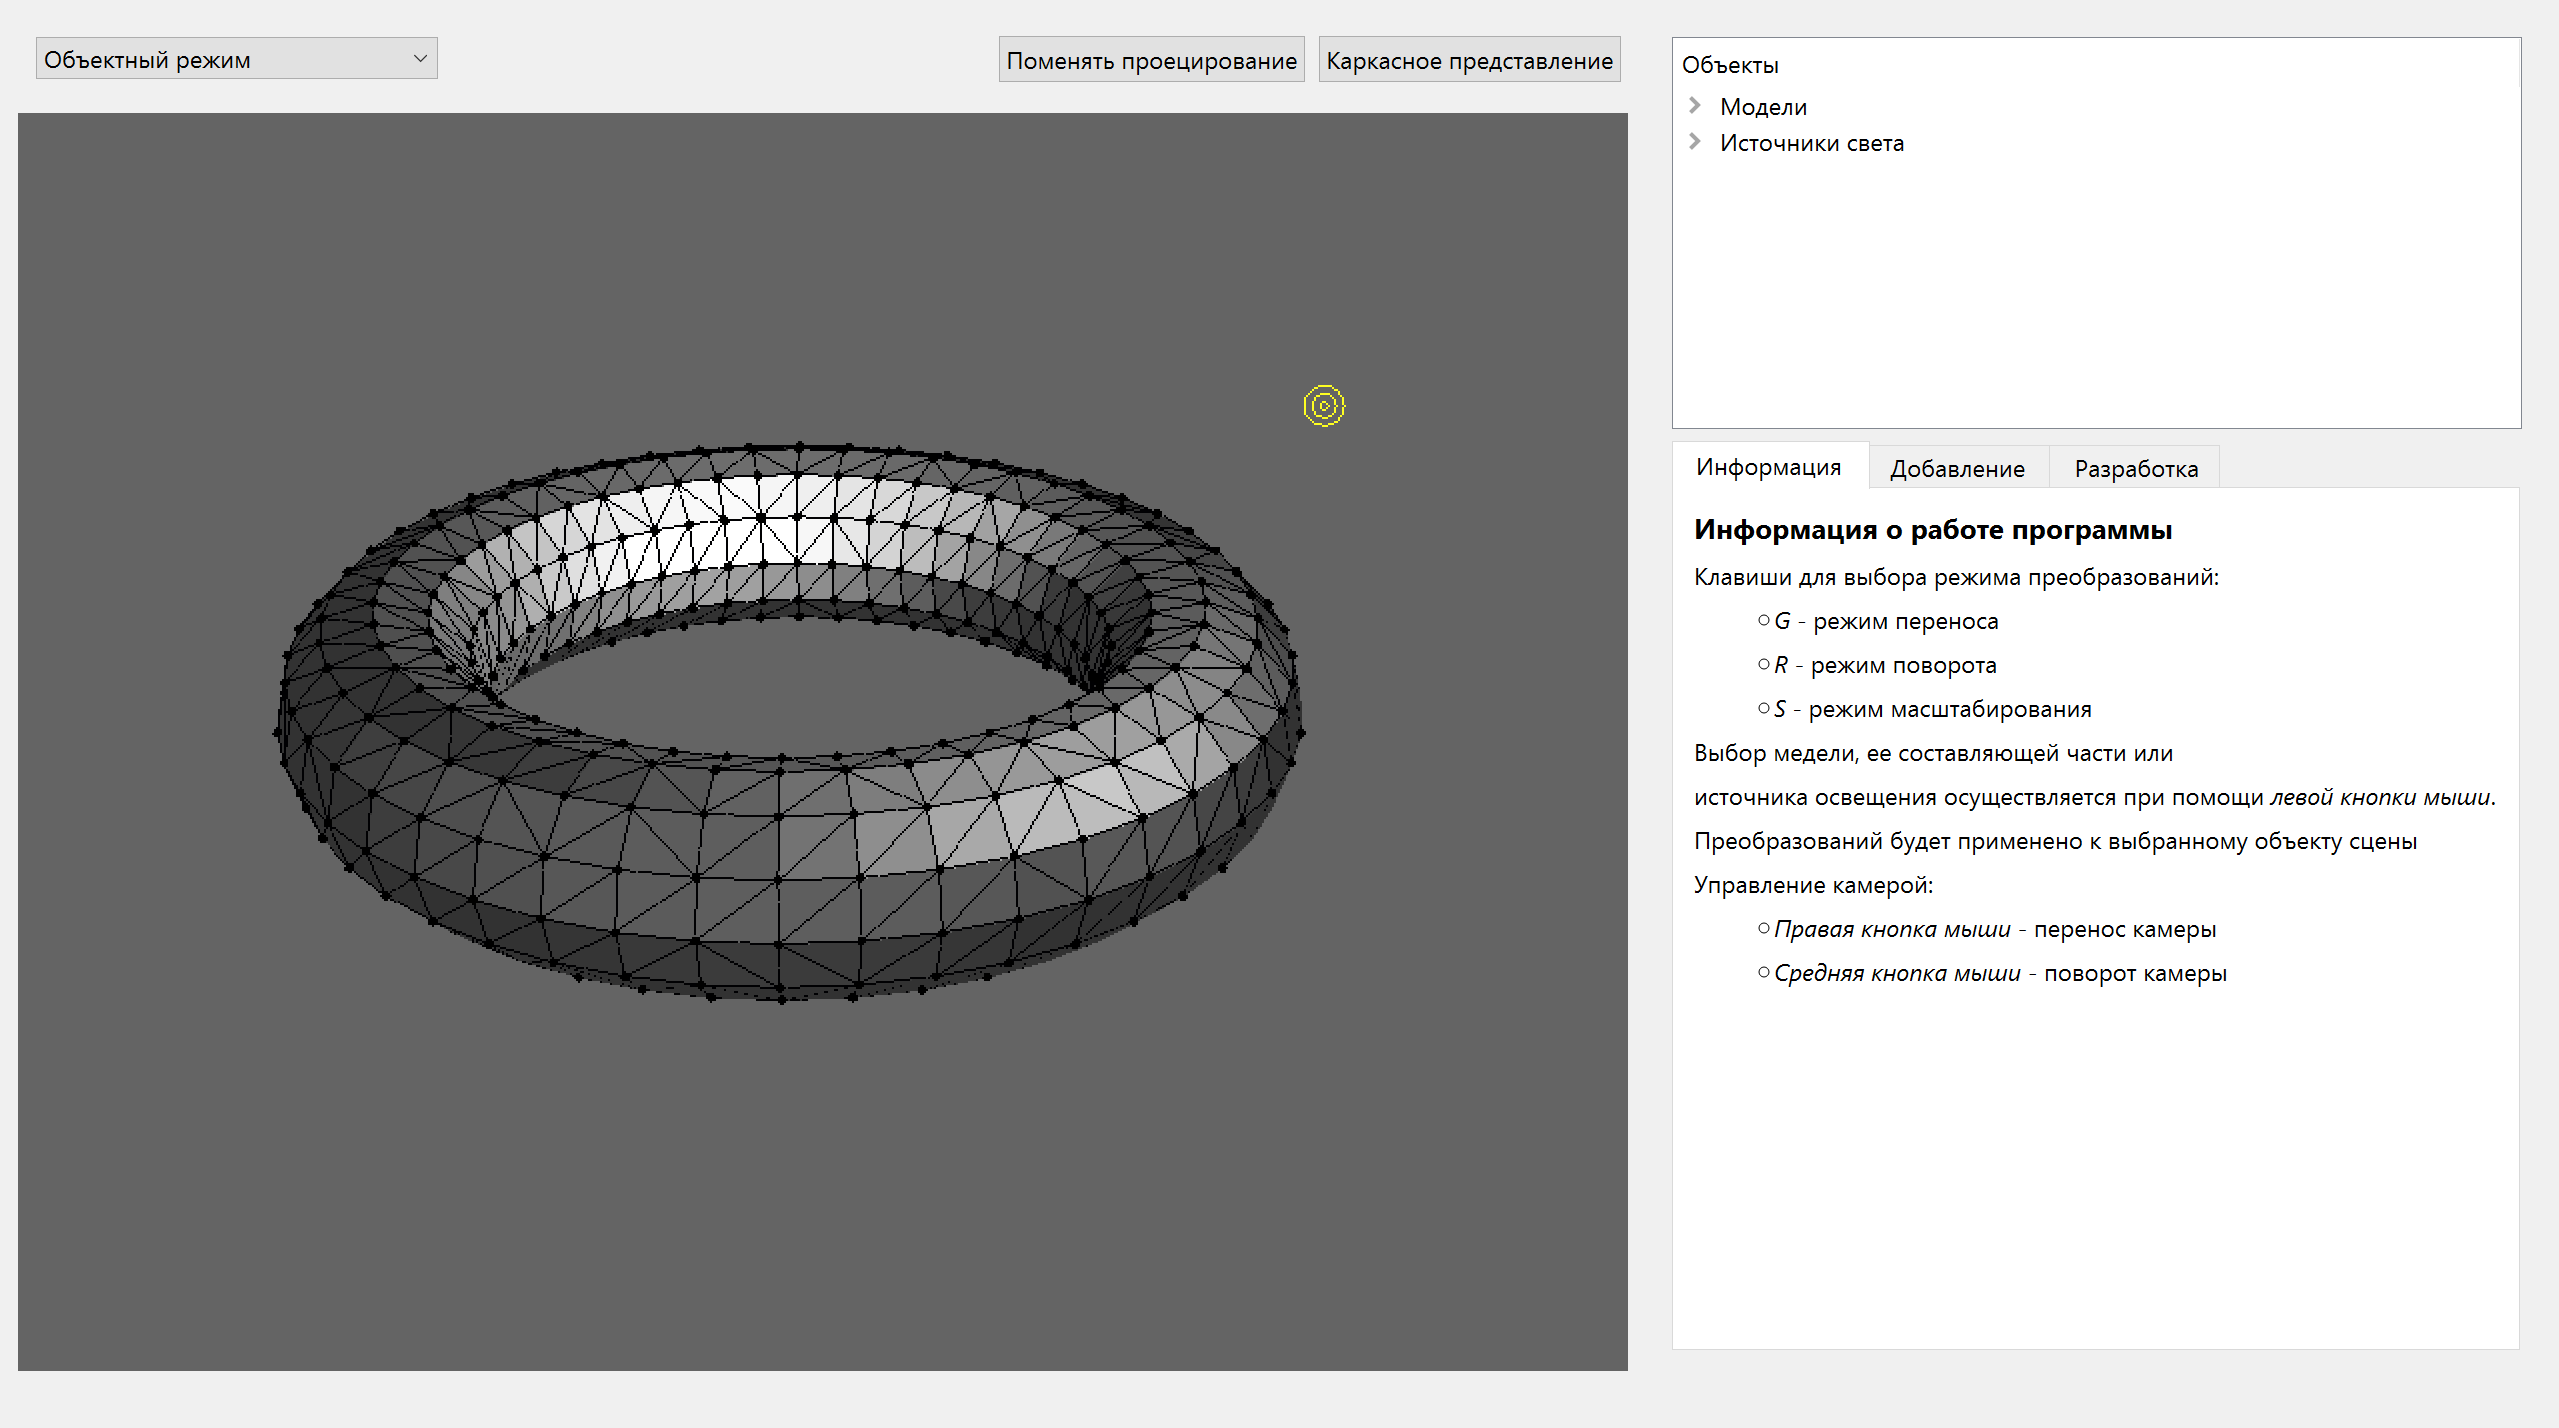
\includegraphics[scale=0.5]{inc/img/interface.png}
	\caption{Основное окно программы}
	\label{fig:interface}
\end{figure} 


\begin{itemize}[label=---]
	\item ПО центру экрана находится виджет, на котором визуализируется сцена;
	\item Справа сверху располагается виджет с наименованиями объектов на сцене;
	\item Справа снизу располагается страничный виджет c тремя вкладками:
	\begin{enumerate}
		\item Информация -- вкладка с информацией об элементах управления;
		\item Добавление (рисунок \ref{fig:add_page}) -- вкладка с кнопками для добавление примитивов на сцену;
		\item Разработка -- служебная вкладка с вспомогательными функциями для отладки программы.
	\end{enumerate}
	\item Сверху располагается <<Комбобокс>> для выбора режима редактирования и кнопки для изменения проекции и представления модели.
\end{itemize}

Интерфейс программы также содержит меню со следующими пунктами:
\begin{itemize}[label=---]
	\item Файл -- позволяет загрузить сцену или модель;
	\item Справка -- отображает справочную информацию о программе.
\end{itemize}

\begin{figure}[h]
	\centering
	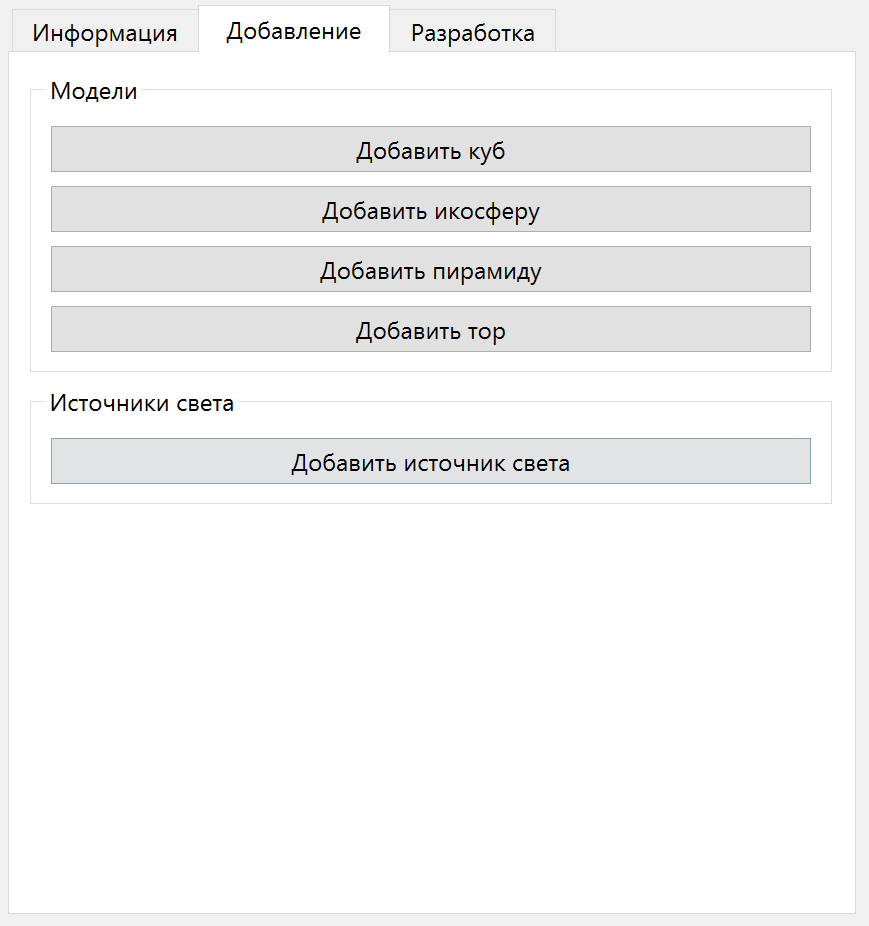
\includegraphics[scale=0.7]{inc/img/add_page.png}
	\caption{Вкладка <<Добавление>>}
	\label{fig:add_page}
\end{figure} 

